%%%%%%%%%%%%%%%%%%%%%%%%%%%%%%%%%%%%%%%%%
% Masters/Doctoral Thesis 
% LaTeX Template
% Version 2.5 (27/8/17)
%
% This template was downloaded from:
% http://www.LaTeXTemplates.com
%
% Version 2.x major modifications by:
% Vel (vel@latextemplates.com)
%
% This template is based on a template by:
% Steve Gunn (http://users.ecs.soton.ac.uk/srg/softwaretools/document/templates/)
% Sunil Patel (http://www.sunilpatel.co.uk/thesis-template/)
%
% Template license:
% CC BY-NC-SA 3.0 (http://creativecommons.org/licenses/by-nc-sa/3.0/)
%
%%%%%%%%%%%%%%%%%%%%%%%%%%%%%%%%%%%%%%%%%

%----------------------------------------------------------------------------------------
%	PACKAGES AND OTHER DOCUMENT CONFIGURATIONS
%----------------------------------------------------------------------------------------

\documentclass[
11pt, % The default document font size, options: 10pt, 11pt, 12pt
%oneside, % Two side (alternating margins) for binding by default, uncomment to switch to one side
english, % ngerman for German
singlespacing, % Single line spacing, alternatives: onehalfspacing or doublespacing
%draft, % Uncomment to enable draft mode (no pictures, no links, overfull hboxes indicated)
%nolistspacing, % If the document is onehalfspacing or doublespacing, uncomment this to set spacing in lists to single
%liststotoc, % Uncomment to add the list of figures/tables/etc to the table of contents
%toctotoc, % Uncomment to add the main table of contents to the table of contents
%parskip, % Uncomment to add space between paragraphs
%nohyperref, % Uncomment to not load the hyperref package
headsepline, % Uncomment to get a line under the header
%chapterinoneline, % Uncomment to place the chapter title next to the number on one line
consistentlayout, % Uncomment to change the layout of the declaration, abstract and acknowledgements pages to match the default layout
]{MastersDoctoralThesis} % The class file specifying the document structure


\usepackage[utf8]{inputenc} % Required for inputting international characters
\usepackage[T1]{fontenc} % Output font encoding for international characters

\usepackage[%
	left     = ``,%
	right    = '',%
	leftsub  = ``,%
	rightsub = ''%
	]{dirtytalk}

\usepackage{mathpazo} % Use the Palatino font by default
\usepackage{xcolor}


\usepackage{caption}
\usepackage{subcaption}


\usepackage[backend=biber,style=authoryear,maxcitenames=1,maxbibnames=99,natbib=true,uniquelist=minyear]{biblatex} % Use the bibtex backend with the authoryear citation style (which resembles APA)

\addbibresource{../Dokument/MA_literatur.bib} % The filename of the bibliography

%\usepackage[autostyle=true]{csquotes} % Required to generate language-dependent quotes in the bibliography

%----------------------------------------------------------------------------------------
%	MARGIN SETTINGS
%----------------------------------------------------------------------------------------

\geometry{
	paper=a4paper, % Change to letterpaper for US letter
	inner=2.5cm, % Inner margin
	outer=3.8cm, % Outer margin
	bindingoffset=.5cm, % Binding offset
	top=1.5cm, % Top margin
	bottom=1.5cm, % Bottom margin
	%showframe, % Uncomment to show how the type block is set on the page
}

\usepackage{amsmath}

%----------------------------------------------------------------------------------------
%	THESIS INFORMATION
%----------------------------------------------------------------------------------------

\thesistitle{Velocity Distribution Functions of Pickup Ions with Ulysses/SWICS} % Your thesis title, this is used in the title and abstract, print it elsewhere with \ttitle
\supervisor{Prof. Dr. Wimmer-Schweingruber} % Your supervisor's name, this is used in the title page, print it elsewhere with \supname
\examiner{} % Your examiner's name, this is not currently used anywhere in the template, print it elsewhere with \examname
\degree{} % Your degree name, this is used in the title page and abstract, print it elsewhere with \degreename
\author{Anne Fischer} % Your name, this is used in the title page and abstract, print it elsewhere with \authorname
\addresses{} % Your address, this is not currently used anywhere in the template, print it elsewhere with \addressname

\subject{} % Your subject area, this is not currently used anywhere in the template, print it elsewhere with \subjectname
\keywords{} % Keywords for your thesis, this is not currently used anywhere in the template, print it elsewhere with \keywordnames
\university{Christian-Albrechts-Universität zu Kiel} % Your university's name and URL, this is used in the title page and abstract, print it elsewhere with \univname
\department{{Institut für Experimentelle und Angewandte Physik}} % Your department's name and URL, this is used in the title page and abstract, print it elsewhere with \deptname
\group{{Arbeitsgruppe Extraterrestrische Physik}} % Your research group's name and URL, this is used in the title page, print it elsewhere with \groupname
\faculty{{Faculty Name}} % Your faculty's name and URL, this is used in the title page and abstract, print it elsewhere with \facname




\AtBeginDocument{
\hypersetup{hidelinks} % uncomment for printing: unolors links and references
\hypersetup{pdftitle=\ttitle} % Set the PDF's title to your title
\hypersetup{pdfauthor=\authorname} % Set the PDF's author to your name
\hypersetup{pdfkeywords=\keywordnames} % Set the PDF's keywords to your keywords
}

\begin{document}

\frontmatter % Use roman page numbering style (i, ii, iii, iv...) for the pre-content pages

\pagestyle{plain} % Default to the plain heading style until the thesis style is called for the body content

%----------------------------------------------------------------------------------------
%	TITLE PAGE
%----------------------------------------------------------------------------------------

\begin{titlepage}
	
\begin{center}
		
	\HRule \\[0.4cm] % Horizontal line
	{\huge \bfseries \ttitle\par}\vspace{0.4cm} % Thesis title
	\HRule \\[1.5cm] % Horizontal line
	
	
	\textsc{\LARGE Master Thesis}\\[8.9cm] % Thesis type
	{\Large \authorname}\\[.2cm] % Author name - remove the \href bracket to remove the link
	{\Large Dezember 2019}\\[1cm] % Date
	
	


	
	\vfill
	

	{\Large \univname\\} % University name
	{\Large \deptname\\\groupname\\[2cm]} % Research group name and department name
	
	\vfill
	
	

	
	\vfill
\end{center}
%\begin{center}
%
%\vspace*{.06\textheight}
%{\scshape\LARGE \univname\par}\vspace{1.5cm} % University name
%\textsc{\Large Master Thesis}\\[0.5cm] % Thesis type
%
%\HRule \\[0.4cm] % Horizontal line
%{\huge \bfseries \ttitle\par}\vspace{0.4cm} % Thesis title
%\HRule \\[1.5cm] % Horizontal line
% 
%\begin{minipage}[t]{0.4\textwidth}
%\begin{flushleft} \large
%\emph{Author:} \\
%{\authorname} % Author name - remove the \href bracket to remove the link
%\end{flushleft}
%\end{minipage}
%\begin{minipage}[t]{0.4\textwidth}
%\begin{flushright} \large
%\emph{Supervisor:} \\
%{\supname} % Supervisor name - remove the \href bracket to remove the link  
%\end{flushright}
%\end{minipage}\\[3cm]
% 
%\vfill
%
%\large
%\groupname\\\deptname\\[2cm] % Research group name and department name
% 
%\vfill
%
%{\large \today}\\[4cm] % Date
%%\includegraphics{Logo} % University/department logo - uncomment to place it
% 
%\vfill
%\end{center}
\end{titlepage}


%----------------------------------------------------------------------------------------
%	ABSTRACT PAGE
%----------------------------------------------------------------------------------------

\begin{abstract}
\addchaptertocentry{\abstractname} % Add the abstract to the table of contents


Pickup ions (PUI) are former neutral atoms that are ionized in the heliosphere. The neutral atom's origin is either the interstellar medium (interstellar PUI) or a source within the heliosphere (inner-source PUI).\\
After ionization, the PUI's velocity distribution function (VDF) is shaped by interaction with the magnetized solar wind plasma. The general idea is that PUI are swept outwards with the solar wind and that their initially anisotropic VDF is rapidly deformed by different processes and conditions within the heliosphere. 
The details of involved mechanisms like e.g. pitch-angle scattering and adiabatic cooling are not completely understood to this day.
A study of the evolution of the VDF helps us to understand the origin of PUI and their neutral seed population and of the underlying effects that shape the VDF.
\\
However, most observations of PUI are limited to 1D reduced velocity measurements in the spacecraft frame. Consequently, they do not allow for interpretations without making assumptions about the underlying VDF.
%The aim is to resolve the VDF in three dimensions and to transform it into the SW frame. 
\\
In this Master thesis I want to develop a method for resolving data measured by the Solar Wind Ion Composition Spectrometer (SWICS) onboard the spacecraft Ulysses in three dimensions.
SWICS is a time-of-flight mass spectrometer that is able to determine the mass, mass-per-charge and energy of ions by independent measurements of the ion's energy-per-charge, time-of-flight and residual energy. Additionally, SWICS provides information on the inflow direction of incident ions by a three-part division of the sensor and a sectorization of Ulysses' spin. 
For translating this information correctly into three-dimensional velocity components it is necessary to consider Ulysses' orientation in space at any time of measurement.
\\
In this work, I utilize a virtual detector to perform a transformation from Ulysses SWICS Pulse-Height Analysis data into three-dimensional velocity components using the example of $\mathrm{He^+}$ PUI.



%.
%\\ \\
%-- Two prominent processes that influence the initial VDF are pitch angle scattering and energy exchange.   \\
%
%-- For understanding a) (transport) processes in the heliosphere and b) origin of the PUI it is necessary to Understand the details of how the VDF evolves\\
%Two prominent processes that may have a significant impact on the VDF are PAS and C., which are not completely understood to this day.
%
%These processes include e.g. pitch-angle scattering and ``cooling'' , which are not completely understood to this day \\
%We utilize this directional information to analyse the Ulysses SWICS PUI data in three dimensions for the first time.
%
%Coordinate Systems are described
%Virtual detector is constructed after the original geometry
%Consider orientation and eigen-velocity of the spacecraft (crazy orbit)
%normalization: phase space density
%
%---------
%Using a virtual detector under consideration of Ulysses' orientation in space we 
%
%we combine this directional information with the orientation of Ulysses
%to obtain 
%
%A virtual detector is utilized to combine absolute velocity measurements with the orientation of the instrument. 
%Kombinieren diese Infos mit der Ausrichtung des SC











\end{abstract}


% Abstract Deutsch
\begin{abstractd}
	Pickup-Ionen (PUI) sind ehemals neutrale Teilchen, die innerhalb der Heliosphäre ionisiert werden. Die Neutralteilchen stammen entweder aus dem interstellaren Medium (interstellare PUI) oder aus einer Quelle innerhalb der Heliosphäre (Inner-Source PUI).\\
	Nachdem die Teilchen ionisiert wurden, wird ihre Geschwindigkeitsverteilungsfunktion (VDF) durch Wechselwirkung mit dem magnetisierten Sonnenwindplasma geformt. Die grundlegende Vorstellung ist, dass die PUI dann mit dem Sonnenwind nach außen strömen und ihre ursprünglich anisotrope VDF durch unterschiedliche Prozesse in der Heliosphäre verformt wird.
	Dabei sind die Details der beteiligten Mechanismen wie z.B. Pitchwinkel-Streuung oder adiabatisches Kühlen bis heute nicht vollständig verstanden.
	Die Untersuchung der VDF-Evolution kann sowohl dazu beitragen den Ursprung der PUI und ihrer zugrundeliegenden Neutralteilchen zu verstehen als auch die Effekte, die ihre VDF formen.\\
	Allerdings sind die meisten PUI-Beobachtungen auf 1D-reduzierte Messungen im Bezugssystem des Spacecrafts beschränkt, weshalb sie nicht interpretiert werden können ohne Annahmen über die zugrundeliegende VDF zu machen.
	\\
	In dieser Masterarbeit soll eine Methode entwickelt werden, mit der man Messdaten des Instruments SWICS (Solar Wind Ion Composition Spectrometer) an Bord des Spacecrafts Ulysses in drei Dimensionen auflösen kann.
	SWICS ist ein Massenflugzeitspektrometer, mit dem durch unabhängige Messungen von Energie-pro\--La\-dung, Flugzeit und Restenergie eines Ions dessen Masse, Masse-pro-Ladung und Energie bestimmt werden kann. Zusätzlich bietet SWICS eine Messung der Einflugrichtung von Ionen aufgrund von einer Dreiteilung des Sensors und einer Sektorisierung von Ulysses' Spin.  
	Um diese Informationen über die Einflugrichtung kor\-rekt in dreidimensionale Geschwindigkeitskomponenten zu überführen muss die Ausrichtung von Ulysses zu jedem Messzeitpunkt betrachtet werden.
	\\
	In dieser Arbeit wird ein virtuellen Detektor verwendet, um den Übergang von Ulysses SWICS \textit{Pulse Height Analysis}-Daten zu dreidimensionalen Geschwindigkeits\-komponenten am Beispiel von $\mathrm{He^+}$ PUI durchzuführen.	
\end{abstractd}

%----------------------------------------------------------------------------------------
%	LIST OF CONTENTS/FIGURES/TABLES PAGES
%----------------------------------------------------------------------------------------

\tableofcontents % Prints the main table of contents

%\listoffigures % Prints the list of figures

%\listoftables % Prints the list of tables

%----------------------------------------------------------------------------------------
%	ABBREVIATIONS
%----------------------------------------------------------------------------------------

%\begin{abbreviations}{ll} % Include a list of abbreviations (a table of two columns)

%\textbf{LAH} & \textbf{L}ist \textbf{A}bbreviations \textbf{H}ere\\
%\textbf{WSF} & \textbf{W}hat (it) \textbf{S}tands \textbf{F}or\\

%\end{abbreviations}


%----------------------------------------------------------------------------------------
%	THESIS CONTENT - CHAPTERS
%----------------------------------------------------------------------------------------

\mainmatter % Begin numeric (1,2,3...) page numbering

\pagestyle{thesis} % Return the page headers back to the "thesis" style

% Include the chapters of the thesis as separate files from the Chapters folder
% Uncomment the lines as you write the chapters

% Chapter Template

\chapter{Introduction} % Main chapter title

\label{chap:intro} % Change X to a consecutive number; for referencing this chapter elsewhere, use \ref{ChapterX}


kurze Übersicht:
was ist das Problem (Fragestellung), wie löse ich das, in dieser Arbeit wird das und das gemacht
(A. etwas ausführlicher wdh.)

Der Phasenraumtransport von PUI wurde bereits sehr detailliert modelliert. Bestätigung durch Messungen hängt aber zurück, da die Messungen häufig auf 1D reduziert sind.
In dieser Arbeit soll ein Tool erstellt werden, das 3d auflösen kann auf Basis von Daten, die bisher nicht ausreichen ausgewertet wurden
Tool bauen anhand for Ulysses/SWICS Daten. SWICS hat grobe Richtungsauflösung (Winkel angeben). 



Warum PUI?
weil breite Verteilung. Ideale Population, um Werkzeuge zu tsten und anzuweneden
(weil räumliche Auflösung halt doch nicht so toll ist: Winkelschritte von...)

PUI differ from solar wind ions by a very non-Maxwellian Velocity Distribution Function. As this distribution is particularly broad, PUI are the perfect candidates for testing the METHOD and being studied with it.



Ulysses
weil viele PUI Studioen darauf aufgebaut haben
kann radiale Entwicklung auflösen




Motivation:
Gloeckler zeigen
Ohne Modellvorstellung kann man anhand dieses Spektrums...
wurde nicht aus einer eindeutigen Verteilung erstellt

Es gibt unendlich viele 3D-Modellfunktionen, die auf 1D reduziert so eine Kurve darstellen (Uneindeutigkeit der reduzierten Daten). Man verliert Informationen. Darum macht es keinen Sinn, 1D zu betrachten, wenn man die Möglichkeit hat, sich 3D anzuschauen. 

***
Zentrale Frage: Phasenraumtransport verstehen
Und die gemachten Modelle, z:B auch Kühlen, verstehen.
9) Trafo
Logisch: Bezugsframe ist der Sonnenwind und kein künstlicher SC-Frame, d.h. wir müssen übergehen. Dafür brauchen wir aber die 3D Informationen

...wie würde das in 3D aussehen?

“Drews 2013: While the assumption of a fully isotropic He+ VDF would allow for the transition from the SC to a SW frame of reference even without knowing the three components of the He+ velocity vector, [...] a non isotropic He+ VDF [...] will result in a significant difference in shape and intensity of the observed spectra between the two frames of refrence,
Man kann in 1D nicht die einzelnen Prozesse unterscheiden, die zu einer bestimmten Verteilung führen
Warum sw frame?\\
Warum brauchen wir 3D? Um das zu entfalten und dann den Frame wechseln zu können.





Gliederung vorstellen


\section{Loose Ends}
Warum sw frame?\\
Warum brauchen wir 3D? Um das zu entfalten und dann den Frame wechseln zu können.
Oder Überkapitel Solar Physics?
\\ \\
Heliosphere: Grenze zu LISM
\\ \\
Solar Wind: Zusammensetzung, schneller und langsamer, high latitudes: less complex, constant in speed \\ \\
B-Feldgleichung
\\ \\
Irgendwohin muss unbedingt Motivation, warum PUIs überhaupt interessant sind zu messen!
\\
PU Process\\ \\\
Instrument that is capable of measuring this distribution: large acceptance in absolute velocity, large variation and resolution in angles
%%%
%-------------------------------------------------------------
%%%

10% Chapter 1

\chapter{Pickup Ions} % Main chapter title

\label{chapter:theory} % For referencing the chapter elsewhere, use \ref{Chapter1} 

%-------------------------------------------------------------



%-------------------------------------------------------------

Pickup ions are created when neutral atoms inside the heliosphere become ionised and are subsequently swept away with the heliospheric magnetic field that is embedded within the solar wind.


\section{The Heliosphere / Introduction}

Oder Überkapitel Solar Physics?
\\ \\
Heliosphere: Grenze zu LISM
\\ \\
Solar Wind: Zusammensetzung, schneller und langsamer, high latitudes: less complex, constant in speed \\ \\
B-Feldgleichung
\\ \\
Irgendwohin muss unbedingt Motivation, warum PUIs überhaupt interessant sind zu messen!
\\
PU Process
%%%
%-------------------------------------------------------------
%%%

\section{Pickup Ions}
A neutral atom inside the heliosphere is only subjected to the gravitational force and radiation pressure of the sun. It is not sensitive to any electromagnetic forces until it becomes ionised by solar ultra-violet radiation, charge exchange with solar wind protons or electron impact (Q?). After ionisation the particle starts interacting with the solar wind plasma. In particular it is forced onto a gyro orbit about the heliospheric magnetic field
that is embedded within the solar wind. As the freshly created ion is swept away with the magnetic field line it is \say{picked up} from its location of ionisation -- a new pickup ion (PUI) has been created.
\\ \\
PUIs were first observed by \citet{moebius_nature_85} with the SULEICA Instrument on the AMPTE spacecraft. The particles measured at $1\,\mathrm{AU}$ were He+ ions of interstellar origin.
\\ \\
Once the particle is ionised, its probability to become ionised another time decreases (Quelle). This characteristic of being only singly charged can help to discriminate PUIs from solar wind ions, that are mostly more often charged (Q?).
\\ \\
PUIs are mostly only single charged. This characteristic can help to distinguish them from solar wind ions of coronal origin which often have been ionized multiple times, if not completely. (Q?)
\\
VDF non-maxwellian, spatial density pattern 
\\ \\
There have been observed several species of PUIs: 
\section{Interstellar Pickup Ions}
Heliosheath, relative motion \\ \\
The neutral part of the LISM can enter the heliosphere as it is not affected by the heliosheath (Todo). Inside the heliosphere the neutrals are guided only by the gravitational force and raOriginofC-Geissdiation pressure of the sun. The neutral particle's species determines how deep it can travel into the heliosphere before it becomes ionized. Species with a higher First Ionization Potential will be able to approach the sun much closer without being ionized. This results in He+ being the dominant PUI species at a solar distance of $1\,\mathrm{AU}$ even if in the LISM the abundance of hydrogen is about 10 times the one of helium.
\begin{itemize}
	\item ionisation process is also dependent on the species
	\item radiation pressure only important for H (and He?). Kepler orbit...
	\item Spatial distribution:\\
	gravitational force and radiation pressure lead to two regions of enhanced density of neutrals (in the ecliptic): Focusing cone and crescent.
	Focusing cone: For species with high FIP (as the others are ionized before and do not reach the downwind side of the sun)
	\item variation of He+ with the solar cycle: Rucinski 2003
	\item H, O and N are depleted in the filtration region (Baranov Malama 1995), Wimmer Skript: even before ioniztion: density is determined by ratio of gravitational force and photon pressure
	\item neutral density determines PUI production rate
\end{itemize}

\section{Inner-source Pickup Ions}
The idea of an additional source for the PUI's neutral seed population was born when \citet{geiss_1995a} measured a global distribution of C+ PUIs with the SWICS instrument on Ulysses. 
Interstellar carbon exists almost exclusively in a single charged state \citep{Frisch} in the LISM. As only neutral atoms can enter the heliosphere it was not expected to find a distinct signature of C+ pickup ions.
However, pickup carbon was observed with about the same ratio as oxygen, of which, in contrast, ~80\% is in a neutral charge state in the interstellar medium.
These findings suggested that there must be another source for neutrals that has its origin somewhere inside the heliosphere. \\
In following studies \citep[e.g.][]{geiss_1995b} there were found also other species like O+ and Ne+ of these, so called, inner-source PUIs.
\\
Inner-source PUIs show a composition that is similar to the one of the solar wind \citep{gloeckler2000_innersource, allegrini_2005} as well as a velocity distribution function that is centered around $w_{SC} \approx 1$ \citep{schwadron_2000} and seems to have thermalized with the solar wind.
\\
Beneath those two characteristics there are other aspects concerning inner-source PUIs, that are still under debate. In particular that is the production mechanism of their neutral seed population.
\citet{allegrini_2005} has summarized current candidates for possible scenarios. Two of those give an explanation for the ion's composition as they directly incorporate solar wind ions in the process:
\begin{itemize}
	\item Solar wind recycling \citep{gloeckler2000_innersource, schwadron_2000}: Absorption of solar wind ions by heliospheric grains and subsequent reemission of neutral atoms
	\item Solar wind neutralization \citep{wimmer_2002}: Solar wind ions penetrate sub-micron-sized dust grains and undergo (partial) neutralization by charge exchange
\end{itemize}
(As this work does not focus on inner-source PUIs in particular...)


\section{VDF}
After the particle has been ionised it is forced onto a gyro motion about the local field line of the heliospheric magnetic field due to the Lorentz force. 
\\ \\
To examine the velocity distribution of PUIs after they have been ionized we need to consider the initial speed $v_{ini}$ of the neutral particle. 
For neutrals from the LISM this is mainly given by the inflow speed $v_{ISM}$ of the local interstellar medium with which they enter the heliosphere. As we don't exactly know about the production mechanism of inner-source PUIs, the following considerations mainly relate to interstellar PUIs.
\citet{schwadron_2015_ibex} obtained $v_{ISM} \approx 25 \,\mathrm{km\,s^{-1}}$ with the IBEX satellite for helium. Considering the acceleration by the sun's gravitational force we have a maximum initial speed of $v_ini \approx 50 \,\mathrm{km\,s^{-1}}$ at $1\,\mathrm{AU}$. Compared to an average solar wind speed of $v_{sw} \approx 400\,\mathrm{km\,s^{-1}}$ one can neglect this initial speed in a first step.

For simplicity we thus consider a neutral particle at rest that becomes ionized by one of the aforementioned processes. The freshly created ion now is subjected to the electromagnetic forces of the solar wind plasma. In particular, it finds itself at a velocity $v_{sw}$ relative to the magnetic field which is convected outwards by the solar wind that is assumed to flow radially outwards. Due to the Lorentz force the PUI starts to gyrate about the magnetic field line on an orbit that is perpendicular to it. \\
When we further consider a magnetic field's orientation that is perpendicular to the solar wind flow, $\vec{B} \perp \vec{v}_{sw}$, the ion's gyration speed is $v_{sw}$ while its guiding center moves together with the field line at a speed of $v_{sw}$ as well.
Thus, the total speed of the PUI ranges between $0\, \mathrm{v_{sw}} $ and $2 \, \mathrm{v_{sw}}$ in a sun frame of reference. \\
As the heliospheric magnetic field lines are shaped like an Archimedean spiral, the so called \textit{Parker spiral}, the assumption of a perpendicular magnetic field only applies when solar wind speed $v_{sw}$ and solar distance $r_\odot$ follow the relation
\begin{align*}
90 ^\circ \approx  arctan \left( \frac{2\pi}{T_\odot \cdot v_{sw}} r_\odot \right)
\end{align*}
with sun's sidereal period $T_\odot \approx 25\,d$ \citep{prlss_2004}.
In other cases, e.g. for solar distances about $1\,\mathrm{AU}$, at which the angle between solar wind and magnet field direction is approximately $45^\circ$, the maximum speed in a sun frame of reference is decreased. In general, the gyration speed is given by
\begin{align*}
todo
\end{align*}
with ... .
\\ \\
The velocity space for a pickup situation with a non-radial magnetic field orientation is shown in figure todo on the right.
The PUI's total velocity consists of the movement of the guiding center (...) and the gyration velocity (...). We note, that in this case there is a relative velocity between the motion of the solar wind bulk and the PUI's guiding center movement. 
\\
However, independent on the magnetic field orientation, every possible velocity space trajectory is part of a sphere with the radius $v_{sw}$ centered around $\vec{v}_{sw}$. That means that, in the frame of the solar wind, the freshly created PUI always moves with a speed that is as fast as the solar wind itself. (todo: Hier w einführen?) 
\\ \\
Instead of a single PUI we can consider an ensemble of PUI's that is injected into the solar wind while the magnetic field orientation is not changing much. For that we expect the VDF to form a ring shape in velocity space, commonly called the "PUI torus VDF" \citep{oka_2002}.
The expected orientation of this highly anisotropic torus VDF depends on the local magnetic field direction and is sketched in figure todo for three different angles.
\\ \\
...thickness that is related (associated) to the neutral's velocity and is very small compared to the radius...\\ \\
Spatial diffusion: chalov Fahr 1998. Signature of plasma parcel in which is was produced doesn't match with the one it is measured in
\\ \\
After the injection, the PUI population is radially carried away with the solar wind. During phase space transport through the heliosphere the PUIs are subjected to multiple processes that are expected to modify the shape of the initial toroidal VDF. However, it is not completely understood how the VDF evolves in detail.
\\ \\
A fast isotropization of the VDF due to pitch-angle scattering was suggested by \citet{vasyl_siscoe_1976} in a theoretical work.
However, observations by e.g. \citet{moebius_98} on $He+$ or \citet{gloeckler_1995} on TODO have shown clear anisotropic features in the measured VDFs.
Following studies (todo) explained these findings with the assumption that the ions would be injected into the sunward hemisphere of velocity space more likely. Ineffective pitch-angle scattering into the antisunward hemisphere thus would result in an radial anisotropy.
\\ \\
Recent observations have emphasized the influence of the magnetic field direction on the measured anisotropy.
Utilising 2D analyses of the velocity space, \citet{oka_2002} and \citet{drews_2015} found that the measured VDF of PUIs is systematically oriented about the direction that is perpendicular to the magnetic field.
Thus, it is believed that the VDF's anisotropic features are remnants of the initial toroidal VDF. (and the pa scattering didnt have enough time to isotropize the distribution)
\\ \\
Furthermore, there are different acceleration and deceleration processes that change the PUI's initial VDF and lead to a diffusion in velocity space.
Under the assumption of an isotropic VDF the PUI population is often treated as an adiabatic gas that is consequently cooled when expanding with the solar wind. This picture, initially suggested by \citet{vasyl_siscoe_1976}, however, must be reviewed due to the doubtful fact of a fully isotropic VDF.
Another cooling mechanism, called the \textit{magnetic cooling}, is due to the magnetic field weakening with solar distance. As the PUIs are swept outwards both their ... and their ...invariant have to be conserved which leads to a decrease in both velocity components (parallel and perpendicular to the magnetic field) and thus to a decrease in total velocity (in the frame of the solar wind).
\\ \\
(focusing (adiabatic invariant) \& Ginzberg Landau (Fahr2008): "magnetic cooling" (auch gute Erklärung: Fahr\&Fichtner2011))
\\ \\
Acceleration of PUIs can be caused by 
acceleration: first and seconf order fermi (verstehen, gründe): eher außen bzw. ehr innen. Außerdem ein Mechanismus, der nicht an einzelne Events gebunden ist, sondern immer vorhanden: Mechanismus für alle Teilchen, power law -5...\\
man kann in der 1D Verteilung beobachten, dass 2vsw exceeded wird
\\ \\
PUI He should be measured throughout the mission as they penetrate the heliosphere until 0.5 AU \citep{gloeckler_1992}
\\ \\ \\
Instrument that is capable of measuring this distribution: large acceptance in absolute velocity, large variation and resolution in angles
\subsection{1D reduced VDF, aim of this work...?}
% Chapter Template

\chapter{Instrumentation} % Main chapter title

\label{ChapterInstrumentation} 

%----------------------------------------------------------------------------------------

%----------------------------------------------------------------------------------------

\section{Ulysses}
The spacecraft Ulysses was a joint NASA/ESA project for studying the heliosphere that orbits the sun from 1990 and ...
Ulysses was the first spacecraft with an out-of-ecliptic orbit. With its special trajectory it was capable of taking in-situ measurements from above the poles of the sun. \\
-- Lifetime \\
-- Scientific goals\\


scientific payload  -- trajectory -- aspect angle (antenna)-- Power: RHU because too far away for solar panels (and radiation belt of Jupiter) -- rotation stabilization
\section{SWICS}
sffsf 
% Chapter Template

\chapter{Data Analysis and Methods} % Main chapter title

\label{Chapter:Data} 

%----------------------------------------------------------------------------------------

%----------------------------------------------------------------------------------------


von den Rohdaten zur 3D VDF
\\ \\
wohin damit? \\ \\
PHA pro Spin...
Ideal / mit Fehlern alpha, beta
\\ , Pile-up, random coincidences/ Schmutztail durch hohe Flüsse
\\
SWICS provides two types of data products from the analogue signals Tof, ESSD and the EPQ-Step.
24-bit



\section{Data products}
PHA words, data transmission

\subsection{Priority weighting}
SWICS performs an on-board mass and mass-per-charge-classification. For every ion with valid measurements the $m$ and $mpq$ are calculated based on the measurements of ESSD, Tof and the particle's EPQ-step using a look-up-table technique.\\
On the one hand these values are used for sorting the ions into predefined boxes in the m-mpq-space which yield in the so-called matrix rate, a second data product that is provided by SWICS.\\
Secondly, and more important for our analysis, the m and mpq information is used to sort every measured ion into one of three priority ranges.

Range, BRW\\ \\
\begin{tabular}{c|c|c}
	%\hline
	Range 0 & $m < 8.7$;  $m_0 : mpq < 3.3$ & $\mathrm{H}$, $\mathrm{He^+}$, $\mathrm{He^{2+}}$; Doubles\\ 
	\hline 
	Range 1 & $m > 8.7$ & Heavier ions \\ 
	\hline 
	Range 2 & $m_0 : mpq > 3.3$ & Doubles \\ 
	%\hline 
\end{tabular} 

\subsection{Detection efficiencies}
Threshold, Doubles...



%
%
%

\section{ET matrices, identification}
Fig. \ref{fig:et_matrix} shows longterm PHA data collected with Ulysses SWICS over two years for EPQ Step 25 (= Energy per charge TODO). For every particle with valid measurements the $\mathrm{E_{SSD}}$ channel is plotted over the ToF channel. As a particle's mass and mass-per-charge is connected to the measured values $EpQ$, $\tau$ and $E_{SSD}$ by equations \ref{eq:swics_set1} --  \ref{eq:swics_set3}, every ion species occupies a distinct position in the so-called \textit{ET-Matrix}. (Counts of different ion species sum up at distinct places in ... space.)


\begin{figure}[h]
	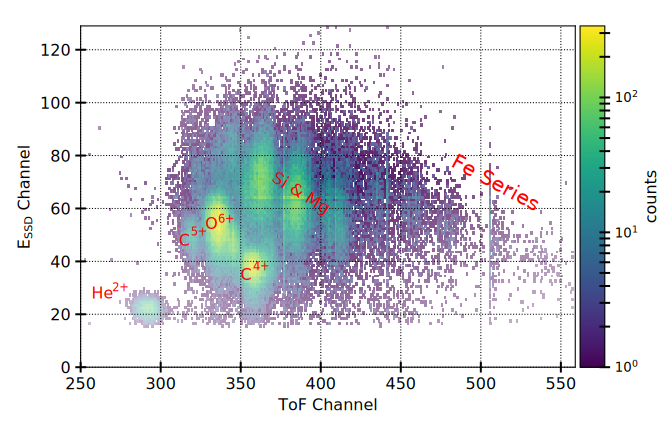
\includegraphics[width=0.9\textwidth]{Figures/et_matrix.pdf}
	\centering
	\caption{test}
	\label{fig:et_matrix}
\end{figure}


\section{Filter He+}
nominal w based on vsw -> solar wind ions rausfiltern
\begin{figure}[h]
	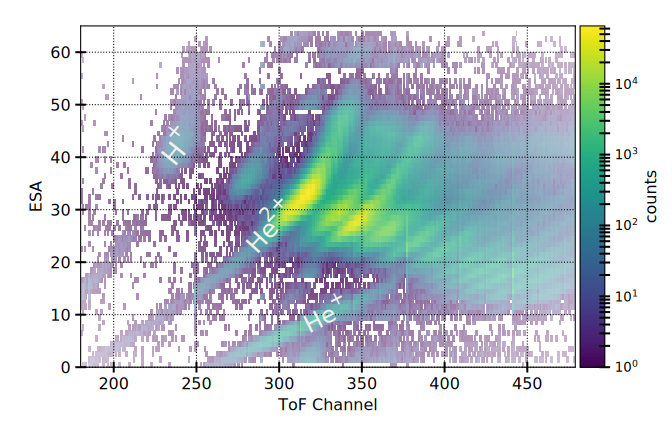
\includegraphics[width=0.9\textwidth]{Figures/epq_all.pdf}
	\centering
	\caption{test}
	\label{fig:epq_all}
\end{figure}


For extracting only the $\mathrm{He^+}$ events from the PHA data we plot the events' energy-per-charge over their measured ToF. 
Teilchen derselben mpq werden auf Kurven $todo$ geortet. Spezies höherer Mpq finden sich auf Kurven mit größeren ToF-Werten. Man kann so z.B. todo, todo und todo identifizieren. Unten ist He gut zu erkennen weil suprathermal. An die suprathermalen $He$-Teilchen schließen sich zu höheren ToF andere Teilchen mit derselben mpq auf der gleichen Kurve an. Weil die Kurven dort enger liegen, kann man He in dem Bereich auch nicht von anderen mit ähnlicher mpq unterscheiden.
We can take advantage of SWICS' on-board priority weighting. We only plot the Range0-events. This roughly cuts out events with $m>8.7$. Nur H, He2+, He+ bleiben übrig als prominente Ionen. Man sieht, dass auch einige schwerere in die Box reinlecken, aber das betrifft nicht die ESA-Steps, in denen Helium auftritt.\\
Man kann jetzt prima per Auge eine Maske legen. Zusätzlich w filtern um eventullen Hintergrund zu unterdrücken...?
Man sieht, dass wir nur Helium-PHAs bis EpQ-Step todo auswerten. Der Grund ist, dass He1+ aufgrund der geringen Masse nicht genug Energie hat, die Triggerschwelle des SSDs zu überschreiten. Somit liegen He1+-Ionen bei höheren ESA-Steps (kleineren Energien pro Ladung) als Double Coincidences vor und taugen nicht für unsere Analyse.
\\
Für alle Jahre. Anzahl: todo
\\ \\
Plots: Nur RNG0, He und He2 gefiltert. In einem (dann nochmal und Fabrsala synchron) oder einzeln?
\\
Irgendwo He+, He++ und Protonen markieren


\subsection{Filter He2+}
für die spätere Kalibrierung (todo: Verweis) brauchen wir eine Spezies, bei der wir davon ausgehen, dass sie sich mit dem SW-Bulk bewegt und die als Triple Coinzidences vorliegt (für die Richtungsinformation). We choose He2+ wegen guter Statistik und auch in Range0. Im Gegensatz zu He1+ auch bei höheren ESA-Steps anzutreffen, weil mehr Nachbeschleunigung durch die höhere Ladung. Dadurch nicht so schnell unter SSD-Threshold. Gleiches Verfahren, einfach ausschneiden. Hier ist es nicht so wichtig, alles mitzubekommen, weil wir anhand von He2+ keine Analyse der VDF durchführen wollen. 
\\
Für alle Jahre. Anzahl: todo
\\ \\
Weitere Daten: vsw von SWOOPS, B-Feld
\\ \\
wie viele Daten bleiben über, wie viele PHA-Worte ca. pro Spin?


%
%
%
\section{Collimator/Detector model}

\subsubsection{Motivation}
Kollimatormodell -- warum eigentlich -- wie umgesetzt?\\ \\
Das Ziel ist, einem gemessenen Teilchen einen v-Vektor zuzuordnen. Eine Sek-Det-Kombi ist aber nicht eindeutig. Ihre Bedeutung hängt davon ab, wohin das Instrument guckt (FoV), von der Eigengeschwindigkeit des SC und davon, wie das SC gerade gedreht ist. Zusätzlich hat der Kollimator eine komplizierte Geometrie, sodass eine analytische Lösung schwierig ist: Also numerische Lösung. \\
Was macht das Modell? -- Ich will das FoV zu jedem Zeitpunkt bestimmen. Ich nehme dafür einzelne Messpunkte auf der originalen Geometrie. Dann gebe ich noch ins Modell, wie das gerade ausgerichtet ist.\\
Berechnet anhand des AA, wohin Sun trigger schaut, wenn getriggert wird und rotiert coll. an entsprechende Position für Sek 0. Ordnet entsorechend andere Sektoren an.
Simuliert FoV durch Punkteraster \\
\subsubsection{Construction}
Originalgeometrie beschreiben\\
Konstruktion durch Detektorpunkte
\subsubsection{From FoV to Vspace}
Übergang FoV -> vSpace:
Richtungsinfo aus FoV
Betrag aus EpQ-Steps
außerdem: Eigengeschwindigkeit Ulysses
\subsubsection{EpQ Schalen}




wählbare Anzahlen nrs\_sec usw. Später schreiben, was verwendet wurde (?) ; Steps vsw, asp Winkel
\\ \\
Geometrie, Aspect Angle: Ausrichtung zu jedem Zeitpunkt bekannt
(FoV) (hierher die Kalibration! Nur damit funktioniert die Ausrichtung)
Wir füllen die einzelnen Bereiche mit verschiedenen möglichen Messpunkten\\ \\
Dann nehmen wir PHA-Worte und können jedem ein gemessenes Volumen im Phasenraum zuordnen (?).
\\
Übergang vspace: Dann weiß ich, welche v-Vektoren möglich gewesen sein können, damit dieses PHA-Wort entstanden ist.
\\ \\
Plots: einzelner Sektor -- einmal alles ohne AA -- einmal alles mit AA

%
\begin{figure}
	\centering
	\begin{subfigure}{.5\textwidth}
		\centering
		\includegraphics[width=1\linewidth]{Figures/col_single_new.pdf}
		\caption{A subfigure}
		\label{fig:sub1}
	\end{subfigure}%
	\begin{subfigure}{.5\textwidth}
		\centering
		\includegraphics[width=1\linewidth]{Figures/col_vspace_normal.pdf}
		\caption{A subfigure}
		\label{fig:sub2}
	\end{subfigure}
	\caption{A figure with two subfigures}
	\label{fig:test}
\end{figure}
%
%
\begin{figure}[h]
	\includegraphics[width=0.5\textwidth]{Figures/col_shells.pdf}
	\centering
	\caption{TODO}
	\label{TODO}
\end{figure}
%%%
%%%
%%%
\subsubsection{Ulysses trajectory, HG system}
\begin{figure}[h]
	\includegraphics[width=1\textwidth]{Figures/HG_coord.pdf}
	\centering
	\caption{TODO}
	\label{TODO}
\end{figure}


\subsubsection{AA motivation}
\begin{figure}[h]
	\includegraphics[width=0.5\textwidth]{Figures/col_aa_marker.png}
	\centering
	\caption{TODO}
	\label{TODO}
\end{figure}
	

\subsubsection{Eigengeschwindigkeit}

\subsubsection{Sunpulse Trigger -- Rotation}


\subsubsection{Calibration Sector}

\subsection{Coordinates}
heliographic, heliocentric? 180 Grad Versatz beschreiben? Drehung mit Eulermatrix
\\ \\
trajectory. \\Orbitdaten gegeben in B.1950... Umrechnung?
\\ \\
verschiedene Koordinatensysteme
\\ \\
durch versch. AA wird unterschiedlicher Teil des v-Raums ausgeleuchtet;
\\ \\
Eigengeschwindigkeit Berechnung (s. Kladde S. 84, 85)
\\ \\ 
TODO:
The orbit itself is described in heliographic coordinates, so a cs that is constant (stable?) with respect to the sun. For describing positions and velocities in the frame of the spacecraft (e.g. AA) we need another cs...
\\ \\
Woher HG Daten und Umrechnung in RTN

\begin{figure}[h]
	\includegraphics[width=1\textwidth]{Figures/RTN_AA_angles.pdf}
	\centering
	\caption{Graphical representation of the RTN coordinate system (not to scale). Shown are the Sun (yellow), the Earth (blue) and the Ulysses spacecraft at a non-specific position on its orbit. $\vec{R}$ is defined as the unit vector along the line-of-sight Sun--Earth, $\vec{T}$ as the normalized cross product $\vec{\omega} x \vec{R}$ with $\vec{\omega}$ the angular velocity of the Sun (yellow vector). $\vec{N}$ completes the right-handed Cartesian system. Also shown is the definition of the aspect angle components $\varphi_{asp}$ and $\vartheta_{asp}$ as they are used in this work. The grey plane depicts the $\vec{R}$--$\vec{T}$ plane. $0 ^\circ < \varphi_{asp} < 90^\circ$ and $-90 ^\circ < \vartheta_{asp} < 0^\circ$ in the shown situation. \textbf{TODO: Zeichnung anpassen: Vektorpfeile, Indizes Winkel; Quelle Ulysses Dingsi}}
	\label{fig:rtn}
\end{figure}
\begin{figure}[h]
	\includegraphics[width=1\textwidth]{Figures/aa_new.pdf}
	\centering
	\caption{The evolution of Ulysses' aspect angle components $\varphi_{asp}$ and $\vartheta_{asp}$ from 1991 to the end of the mission are shown. The aspect angle is the angle between the line-of-sight Ulysses--Sun and the orientation of Ulysses' spin axis. A constantly changing aspect angle results from the fact that the spacecraft's antenna, that is nearly parallel with the spin-axis, has to point towards Earth all the time. Particularly large aspect angles occur during the three fast latitude scans around 1995, 2001 and 2007. Here, Ulysses' distance to Sun and Earth is at a minimum. \textbf{Also shown is the... (todo: raus aus der Zeichnung?)} }
	\label{fig:aa}
\end{figure}
%

%
\subsubsection{RTN Coordinate System}
For dealing with Ulysses' trajectory data it is useful to work with \textit{radial-tangential-normal} coordinates. The RTN coordinate system is defined relative to a moving object in the heliosphere -- in this case the spacecraft, Ulysses, and is centered at the sun. A graphical representation on the system can be found in fig. \ref{fig:rtn}. The unit vectors are $\vec{R}$, $\vec{T}$ and $\vec{N}$, where $\vec{R}$ points radially outward from the sun to the current position of the spacecraft. $\vec{T}$ is defined as the normalized cross product of the Sun's angular velocity $\vec{\omega}$ and $\vec{R}$. $\vec{N}$ completes the right-handed Cartesian coordinate system. Consequently, the RTN system is not defined for a spacecraft's position right above one of the Sun's poles as the cross product $\vec{\omega} x \vec{R}$ is zero here. Nevertheless we do not have to worry about this fact as not even Ulysses crosses the poles directly (todo: Verweis?).
\subsubsection{Calculation of the Aspect Angle}
The aspect angle is measured from the line-of-sight Ulysses--Sun (that is $\vec{R}$) to the line-of-sight Ulysses--Earth. To describe this angle uniquely for any moment, we need two spherical coordinates $\varphi_{asp}$ and $\vartheta_{asp}$ based on the RTN system. As shown in fig. \ref{fig:aa}, $\varphi_{asp}$ is measured in the $\vec{R}$--$\vec{T}$ plane between $-\vec{R}$ and the projection of the line-of-sight from Ulysses to the Earth into this plane. $\varphi_{asp}$  is $0^\circ$ for directions along $-\vec{R}$, that is the line-of-sight from Ulysses to the Sun and increases to positive values towards $-\vec{T}$. $\vartheta_{asp}$ is the angle between the projection of the line-of-sight from Ulysses to the Earth into the $\vec{R}$--$\vec{T}$ plane and the line-of-sight itself. It is defined as $0^\circ$ for directions that lie within the $\vec{R}$--$\vec{T}$ plane and $+90^\circ$ for directions along $\vec{N}$.\\
(Todo: Lars fragen, ob die genaue Rechnung hier rein muss, Kladde S. 79)
For the calculation of the aspect angle we used the Ulysses trajectory data (Verweis ... TODO) and Earth trajectory data in heliographic coordinates on a daily basis from \citet{nasa-earth-coord} and converted both to RTN coordinates. In fig. \ref{fig:aa} both components $\varphi_{asp}$ and $\vartheta_{asp}$ as well as the \textit{flat} aspect angle $\alpha$ with  $\alpha = \arccos(\cos{\varphi_{asp}}) + \arccos(\cos{\vartheta_{asp}}) -1$ are shown over the time of the mission. $\varphi_{asp}$ varies in the range from $\sim - 25^\circ$ to $\sim 42^\circ$ and $\vartheta_{asp}$ in a range from $\sim - 30^\circ$ to $\sim 17^\circ$. Large angles occur especially around the three fast latitude scans, i.e. when Ulysses is at its perihelion and has the smallest distance to Sun and Earth.\\
(Todo? Beschreiben, dass ich $\alpha$ mit dem Datenprodukt SPE verglichen habe?)














%
\subsection{Calibration}
\subsubsection{Calibration AA}
\begin{figure}[h]
	\includegraphics[width=0.5\textwidth]{Figures/hist_det_sec_aa_90days2001}
	\centering
	\caption{TODO}
	\label{TODO}
\end{figure}
Plots: \\ 
Verweis auf AA-Plot oben: Dazu Hist-Det -- dann Schemazeichnung SunPulser, dazu Problem irgendwie zeigen
\\ \\
zeigen, dass mit größeren AA vermehrt äußerer Detektor angesprochen wird; 
\\ \\
Problem: sectors are not triggered uniformly (?). Every spin sector 0 is triggered newly. koplanare Lage der drei Vektoren: Spinachse, Sensor, SC-Sun, \textit{when sun crosses the ...plane of the SC}\\
Allover Blick: Sector, der gegnüber liegt, sollte besonders prominent sein
\\ \\
Kalibrierung: He2+, Det-Sec-Histogramme -- Suche nach Sek 0
\\ Hiscale Paper: Sensoren sind umgebaute Albedo-Sensoren
\\ \\
(...) For verifying this angle we use a species for which we know the direction of velocity. That is He2+ that we assume to be flowing radially with the solar wind
\\ \\
Kalibration Detektoren: Für große AA zeigen, dass äußerer Det angesprochen wird
\\ \\
Kalibration Sektoren: Nur bei sehr großen AA möglich (äußerer od. mittlerer Detektor), weil beim inneren der Bulk auf allen landet.
\\ \\
Sektorgeschichte, Sunpulser...


%
%
%
\section{VDF}
Zweifache Beschränkung im w-Space: Bei kleinem w: keine hohen Steps (kleine Geschwindigkeiten) durch das unter-den-Threshold-Rutschen (deshalb können wir auch keinen langsamen SW untersuchen). Bei hohem w: Ende der Schalen (Step 0: 1708.5 km/s)
%
\subsection{Velocity Space Coverage}
vom FoV zum Vspace: Invertieren $\Rightarrow$ Akzeptanz im V-Raum

%
\subsection{Phasenraumnormierung}
Mittlere Phasenraumdichte in einem Bin, in den zwei Instrumentenbins A und B reingehen:
(differential PSD)
\begin{align}
\bar{\rho} = \frac{N_A + N_B}{\frac{N_A}{N_{A,ges}} V_A + \frac{N_B}{N_{B,ges}} V_B }
\end{align}
Dabei ist $N_i$ die Anzahl der Hits, die im Messbin gelandet sind und $N_{i,ges}$ die gesamte Anzahl an Bins. Hits heißt GEsamtcounts durch Detektoranzahl. Eigentlich gebe ich statt $N_i$ $N_i \cdot Detektoranzahl$ rein, aber das kürzt sich ja raus.\\ \\
Effizienz und Sektorgewichte dazu:\\
Allg.:
\begin{align*}
\rho = \frac{N \cdot brw}{V \cdot Eff}
\end{align*}
Und dann
\begin{align}
\bar{\rho} = \frac{N_A + N_B}{\frac{N_A}{N_{A,ges}} \frac{V_A \cdot eff_A}{brw_A} + \frac{N_B}{N_{B,ges}} \frac{V_B \cdot eff_B}{brw_B} }
\end{align}
Unsicherheit EpQ: Delta v. Rechnung fehlerfortpflanzung Kladde S. 84


%
%
%
\section{Und dann so}
Ich hab jetzt ein Set von v-Komponenten pro PHA-Event. Daraus kann ich berechnen:
(mit: In Komponenten aufgeteilt kann man jetzt Geschwindigkeit im SW-frame berechnen, indem man vsw in R-Richtugn abzieht)
\begin{itemize}
	\item Betrag im SW frame
	\item Winkel im w-space (SW frame)
\end{itemize}
B-Feld. Von welchem Instrument? auch RTN-System. Genauso Winkel berechnet.\\
1-min-Mittel (Gyroradius Zeit zeigen) und entsprechend EpQ-Steps den PHAs zugeordnet.


%
%
%
\section{Results}
\subsection{Slices}
\subsection{Skymaps}
\subsection{1D}



%
%
%
\section{Outlook}
\begin{itemize}
	\item Efficiency müsste genau bestimmt werden: Dabei berücksichtigen, welcher Anteil unter den Threshold wandert. Evtl. überschätzen wir die Eff., wenn wir die interpolierten Werte von ACE/SWICS nehmen.
	\item B-Feld-spezifische Untersuchung: Torus
	\item Radialabhängigkeit: adiabatic Cooling, PA-Scattering

\end{itemize}







\subsection{Loose Ends}
\begin{itemize}
	\item andere Daten: B, vsw (Swoops: als vsw wird Protonengeschw. genommen. Ist das überhaupt richtig, ist das der Referenzframe? Und Annahme, dass vsw rein radial ist)
	\item Die Sache mit dem BRW ab 2003
\end{itemize}

% Chapter Template

\chapter{Results} % Main chapter title

\label{chap:results} % Change X to a consecutive number; for referencing this chapter elsewhere, use \ref{ChapterX}
The solar wind speed data is taken from the instrument Ulysses SWOOPS (todo: Quelle)\\
$v_{sw}$ is assumed to stream only radial for this work.\\
\textbf{Steps vsw} \\ \\

\begin{itemize}
	\item Betrag im SW frame
	\item Winkel im w-space (SW frame)
\end{itemize}

%B-Feld. Von welchem Instrument? auch RTN-System. Genauso Winkel berechnet.
%1-min-Mittel (Gyroradius Zeit zeigen) und entsprechend EpQ-Steps den PHAs zugeordnet.
\clearpage
%
%
%
Todo:\\
Schreiben, dass die velocity Akzeptanzpunkte mit den anteilmäßigen Counts histogrammiert werden? Vielleicht auch ins Data-Kapitel, weil das mit der Normierung gemacht wird...? Sind die Counts überhaupt durch n geteilt?
\\ \\
Here we present the results of the procedure described in chapter \ref{chapter:data}. For creating HE+ VDs from He+ SWICS PHA data we synchronize the selected data (s. \ref{chapter:instrumentation} (triple coincidences) with the SC AA, eigen-velocity and solar wind speed.
This gives us directionally resolved counts from the observed phase space volume.
\\
An example for todo days bla is shown in fig. \ref{fig:counts_50}. Here we histogrammed the counts by utilizing cartesian $w_R$, $w_T$ and $w_N$ bins in solar wind frame. Shown are counts in the $w_T - w_N$ plane from a ``slice'' that has been cut out in $w_R$ direction. The orientation of such a cut is sketched in fig. \ref{fig:sketch_slice_R}. In fig. \ref{fig:counts_50} counts within the range $0.3 <= w_R < 0.5$ have been summarized for each $w_T - w_N$ bin.

(D.h. bei vsw ...)



Dividing the counts by the integrated phase space volume for the observed time, which is binned in the same way and shown in fig. \ref{fig:norm_50}, gives the resulting phase space density, s. fig. \ref{fig:psd_50}.

When Comparing the three figures one can see a change in shape between PSV and PSD bzw. Counts. The PSD doesnt cover als of the scanned PSV and is still a round shape but not as symmetrical as the PSV: We didnt observe HE+ PUIs over all the observed psv but only a distinct central volume.


(In fact a sphere! Nicht darstellbar, deshalb scheibchenweise of width $\Delta w = 0.2$  im Anhang. Man sieht hier außerdem coverage...)


2. peak (not central) in Counts and Norm because of AA: where did we look most... vanishes by normalization... no physics but an artificial effect of the measurement

3. psd: majority streams central in this example

4. (?) ring in norm due to psv auf anderen Schalen; da größere Volumina wegen v





noch einen anderen Fall zeigen: anderer Zeitraum, anderes Ergebnis:
Hier sorgt die Normalisierung dafür, dass ein angebliches Ringfeature verschwindet. Auch hier majority radial.

-- andere Schnitte
außerdem noch T und N Schnitt möglich


Ergebnis kann man in noch in anderen Pr. zeigen:
andere Projektionen:
--- Skymap

--- 1D






\clearpage
\subsection{Slices}


%%% R %%%

\begin{figure}[h]
	\includegraphics[width=.4\textwidth]{Figures/slice_R2.pdf}
	\centering
	\caption{todo}
	\label{fig:sketch_slice_R}
\end{figure}

\begin{figure}[h]
	\includegraphics[width=.8\textwidth]{Figures/cart_50_counts_R.pdf}
	\centering
	\caption{todo}
	\label{fig:counts_50}
\end{figure}

\begin{figure}[h]
	\includegraphics[width=.8\textwidth]{Figures/cart_50_norm_R.pdf}
	\centering
	\caption{todo}
	\label{fig:norm_50}
\end{figure}

\begin{figure}[h]
	\includegraphics[width=.8\textwidth]{Figures/cart_50_ps_R.pdf}
	\centering
	\caption{todo}
	\label{fig:psd_50}
\end{figure}

\begin{figure}
\includegraphics[scale=.28]{Figures/cart_lang_R_counts.pdf}
\includegraphics[scale=.28]{Figures/cart_lang_R_norm.pdf}
\includegraphics[scale=.4]{Figures/cart_lang_R_psd.pdf}
\end{figure}



%%% T %%%
\begin{figure}[h]
	\includegraphics[width=.4\textwidth]{Figures/slice_T2.pdf}
	\includegraphics[scale=.45]{Figures/slice_psd_T.pdf}
	\centering
	\caption{todo}
	\label{fig:sketch_slice_T}
\end{figure}

%%% N %%%

\begin{figure}[h]
	\includegraphics[width=.4\textwidth]{Figures/slice_N2.pdf}
	\includegraphics[scale=.45]{Figures/slice_psd_N.pdf}
	\centering
	\caption{todo}
	\label{fig:sketch_slice_N}
\end{figure}


%
%
%
\clearpage
\subsection{Skymaps}
\begin{figure}[h]
	\includegraphics[width=1\textwidth]{Figures/sky_counts.pdf}
	\centering
	\caption{todo}
	\label{fig:todo}
\end{figure}
\begin{figure}[h]
	\includegraphics[width=1\textwidth]{Figures/sky_norm.pdf}
	\centering
	\caption{todo}
	\label{fig:todo}
\end{figure}
\begin{figure}[h]
	\includegraphics[width=1\textwidth]{Figures/sky_ps.pdf}
	\centering
	\caption{todo}
	\label{fig:todo}
\end{figure}
%
%
%
\clearpage
\subsection{1D}

\begin{figure}[h]
	\includegraphics[width=.8\textwidth]{Figures/1D.pdf}
	\centering
	\caption{todo}
	\label{fig:todo}
\end{figure}
%
%
%
\clearpage
\section{Loose Ends}
\begin{itemize}
	\item andere Daten: B, vsw (Swoops: als vsw wird Protonengeschw. genommen. Ist das überhaupt richtig, ist das der Referenzframe? Und Annahme, dass vsw rein radial ist)
	\item Die Sache mit dem BRW ab 2003
	\item Englisch: Relativpronomen, Kommasetzung, British/American
	\item $\mathrm{He^{+}}$ einheitlich, mathrm
	\item Tempus?
	\item kursiv / nicht kursiv wie war das nochmal
	\item spinrate drin?
\end{itemize}
 
% Chapter Template

\chapter{Conclusion} % Main chapter title

\label{chap:concl} % Change X to a consecutive number; for referencing this chapter elsewhere, use \ref{ChapterX}

aim: directional resolution of velocity of incident He ions
SWICS data in its entirety
together with
Ulysses position and orientation  

%----------------------------------------------------------------------------------------
%	THESIS CONTENT - APPENDICES
%----------------------------------------------------------------------------------------

\appendix % Cue to tell LaTeX that the following "chapters" are Appendices

% Include the appendices of the thesis as separate files from the Appendices folder
% Uncomment the lines as you write the Appendices
% Appendix Template

\chapter{PSD -- Sequence} % Main appendix title

\label{AppendixX} % Change X to a consecutive letter; for referencing this appendix elsewhere, use \ref{AppendixX}

%%%%%%%%%%%%%%%%%%%%%%%%%%%


\begin{figure}[h]
	%\includegraphics[width=0.5\textwidth]{Figures/PLOT_EIGEN_VELOCITY.pdf}
	\includegraphics[width=1.\textwidth]{Figures/slices_50_-5.pdf}
	\centering
	\caption{todo}
	\label{fig:todo}
\end{figure}

\begin{figure}[h]
	%\includegraphics[width=0.5\textwidth]{Figures/PLOT_EIGEN_VELOCITY.pdf}
	\includegraphics[width=1.\textwidth]{Figures/slices_50_-3.pdf}
	\centering
	\caption{todo}
	\label{fig:todo}
\end{figure}

\begin{figure}[h]
	%\includegraphics[width=0.5\textwidth]{Figures/PLOT_EIGEN_VELOCITY.pdf}
	\includegraphics[width=1.\textwidth]{Figures/slices_50_-1.pdf}
	\centering
	\caption{todo}
	\label{fig:todo}
\end{figure}

\begin{figure}[h]
	%\includegraphics[width=0.5\textwidth]{Figures/PLOT_EIGEN_VELOCITY.pdf}
	\includegraphics[width=1.\textwidth]{Figures/slices_50_1.pdf}
	\centering
	\caption{todo}
	\label{fig:todo}
\end{figure}

\begin{figure}[h]
	%\includegraphics[width=0.5\textwidth]{Figures/PLOT_EIGEN_VELOCITY.pdf}
	\includegraphics[width=1.\textwidth]{Figures/slices_50_3.pdf}
	\centering
	\caption{todo}
	\label{fig:todo}
\end{figure}

\begin{figure}[h]
	%\includegraphics[width=0.5\textwidth]{Figures/PLOT_EIGEN_VELOCITY.pdf}
	\includegraphics[width=1.\textwidth]{Figures/slices_50_5.pdf}
	\centering
	\caption{todo}
	\label{fig:todo}
\end{figure}

\begin{figure}[h]
	%\includegraphics[width=0.5\textwidth]{Figures/PLOT_EIGEN_VELOCITY.pdf}
	\includegraphics[width=1.\textwidth]{Figures/slices_50_7.pdf}
	\centering
	\caption{todo}
	\label{fig:todo}
\end{figure}

\begin{figure}[h]
	%\includegraphics[width=0.5\textwidth]{Figures/PLOT_EIGEN_VELOCITY.pdf}
	\includegraphics[width=1.\textwidth]{Figures/slices_50_9.pdf}
	\centering
	\caption{todo}
	\label{fig:todo}
\end{figure}

\begin{figure}[h]
	%\includegraphics[width=0.5\textwidth]{Figures/PLOT_EIGEN_VELOCITY.pdf}
	\includegraphics[width=1.\textwidth]{Figures/slices_50_11.pdf}
	\centering
	\caption{todo}
	\label{fig:todo}
\end{figure}


%\include{Appendices/AppendixA}
%----------------------------------------------------------------------------------------
%	BIBLIOGRAPHY
%----------------------------------------------------------------------------------------

\printbibliography[heading=bibintoc]

%----------------------------------------------------------------------------------------


%----------------------------------------------------------------------------------------
%	DECLARATION PAGE
%----------------------------------------------------------------------------------------

\begin{declaration}
	\addchaptertocentry{\authorshipname} % Add the declaration to the table of contents

Hiermit erkläre ich, dass ich die vorliegende Masterarbeit selbständig und lediglich unter Benutzung der angegebenen Quellen und Hilfsmittel verfasst habe. Ferner versichere ich, dass die vorliegende Arbeit noch nicht im Rahmen eines anderen Prüfungsverfahrens eingereicht wurde. \\[1cm]
	
	\noindent Ort, Datum:\\
	\rule[0.5em]{25em}{0.5pt} % This prints a line for the signature
	\\[0.5cm]
	\noindent Unterschrift:\\
	\rule[0.5em]{25em}{0.5pt} % This prints a line to write the date
\end{declaration}


%----------------------------------------------------------------------------------------
%	ACKNOWLEDGEMENTS
%----------------------------------------------------------------------------------------

%\begin{acknowledgements}
%	\addchaptertocentry{\acknowledgementname} % Add the acknowledgements to the table of contents
%	The acknowledgments and the people to thank go here, don't forget to include your project advisor\ldots
%\end{acknowledgements}


\end{document}  
